\documentclass[tikz, border=10pt]{standalone}
\usepackage{xcolor}
\usetikzlibrary{calc}

\definecolor{purple1}{RGB}{148, 0, 211}
\definecolor{green1}{RGB}{0, 150, 80}

\begin{document}
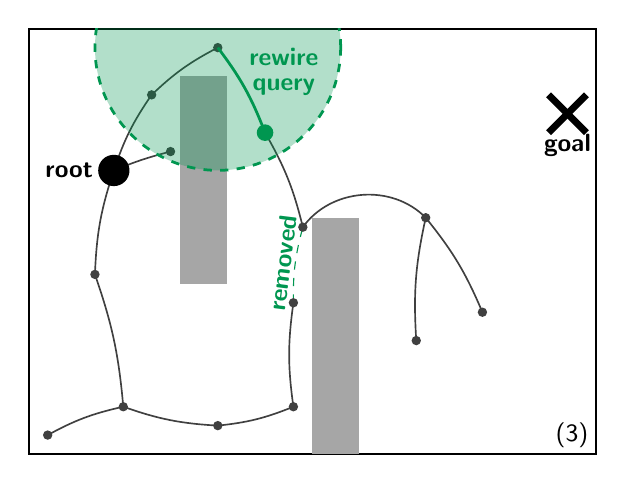
\begin{tikzpicture}[
    scale=1.2,
    obstacle/.style={fill=black!35, draw=none},
    tree node/.style={circle, fill=black!75, inner sep=1.2pt},
    tree edge/.style={draw=black!75, semithick},
    root node/.style={circle, fill=black, inner sep=4pt},
    label font/.style={font=\sffamily\bfseries\small}
]

    % 1. Outer Bounding Box
    \draw[thick] (0,0) rectangle (6,4.5);
    \node[font=\sffamily\small] at (5.75, 0.2) {(3)};

    % 2. Obstacles (Top & Bottom Gray Blocks)
    \fill[obstacle] (1.6, 1.8) rectangle (2.1, 4.0); % Top obstacle
    \fill[obstacle] (3.0, 0.0) rectangle (3.5, 2.5); % Bottom obstacle

    % 3. Tree Nodes & Edges (RRT Structure)
    % Coordinates
    \coordinate (root) at (0.9, 3.0);
    \coordinate (n0)   at (1.5, 3.2);
    \coordinate (n1)   at (1.3, 3.8);
    \coordinate (n2)   at (0.7, 1.9);
    \coordinate (n3)   at (1, 0.5);
    \coordinate (n4)   at (0.2, 0.2);
    \coordinate (n5)   at (2, 0.3);
    \coordinate (n6)   at (2.8, 1.6);
    \coordinate (n7)   at (2.8, 0.5);
    \coordinate (n8)   at (2.9, 2.4);
    \coordinate (n9)   at (2.5, 3.4);
    \coordinate (n10)   at (4.2, 2.5);
    \coordinate (n11)   at (4.1, 1.2);
    \coordinate (n_new)   at (2, 4.3);
    \coordinate (purple_node) at (4.8, 1.5);

    % Straight Edges
    %\draw[tree edge] (root) -- (n1);

    % Straight Edges
    \draw[tree edge] (root) to[bend left=4] (n0);
    \draw[tree edge] (root) to[bend left=8] (n1);
    \draw[tree edge] (root) to[bend right=8] (n2);
    \draw[tree edge] (n2) to[bend left=7] (n3);
    \draw[tree edge] (n3) to[bend right=8] (n4);
    \draw[tree edge] (n3) to[bend right=8] (n5);
    \draw[tree edge] (n5) to[bend right=8] (n7);
    \draw[tree edge] (n6) to[bend right=8] (n7);
    \draw[green1, dashed] (n6) to[bend left=8]
        node[midway, above=-2pt, sloped, font=\sffamily\bfseries\small] {removed} (n8);
    \draw[tree edge] (n8) to[bend right=8] (n9);
    \draw[tree edge] (n10) to[bend left=8] (purple_node);
    \draw[tree edge] (n10) to[bend right=8] (n11);
    \draw[tree edge] (n1) to[bend left=8] (n_new);
    \draw[tree edge] (n8) to[bend left=50] (n10);
    % Curved Connection over Middle Obstacle
    %\draw[tree edge] (n8) .. controls (2.6, 3.5) and (4.0, 3.5) .. (n10);

    % Draw Nodes
    \foreach \n in {n0, n1, n2, n3, n4, n5, n6, n7, n8, n9, n10, n11, n_new, purple_node} {
        \node[tree node] at (\n) {};
    }

    % 4. Root Node & Label
    \node[root node] at (root) {};
    \node[label font, left=4pt] at (root) {root};

    % 5. Goal Marker & Label
    \coordinate (goal) at (5.7, 3.6);
    \draw[line width=2.5pt, black] ($(goal)+(-0.2,-0.2)$) -- ($(goal)+(0.2,0.2)$);
    \draw[line width=2.5pt, black] ($(goal)+(-0.2,0.2)$) -- ($(goal)+(0.2,-0.2)$);
    \node[label font, below=4pt] at (goal) {goal};

    % 6. New Sample Neighborhood Query
    \coordinate (circle_center) at (n_new);
    
    % Dashed Search/Neighborhood Circle
    \begin{scope}
        \clip (0,0) rectangle (6,4.5);
        \draw[
            green1,
            line width=1pt,
            dashed,
            fill=green1,
            fill opacity=0.3
        ] (circle_center) circle (1.3cm);
    \end{scope}
    \draw[thick] (6,0) -- (6,4.5);

    % New Sample
    \fill[green1] (n9) circle (2.5pt);

    % Neighborhood query connections to nearby tree nodes
    \draw[green1, line width=1pt] (n_new) to[bend left=8] (n9);

    % Neighborhood Query Label
    \node[green1, font=\sffamily\bfseries\small, align=center, anchor=north]
        at (2.7, 4.4) {rewire\\[-2pt]query};

\end{tikzpicture}
\end{document}